\documentclass{article}
\textwidth=6in
\hoffset=0in
\voffset=0in


\usepackage[a4paper, total={6in, 8in}]{geometry}
\usepackage{amsmath}
\usepackage{amssymb}
\usepackage{stmaryrd}
\usepackage{graphicx}

\usepackage{tikz}
\usetikzlibrary{automata, arrows}
\tikzset{initial text={}}

\usepackage{pifont}
\usepackage{amssymb}
\usepackage{gensymb}
\usepackage{ngerman}
\usepackage[ampersand]{easylist}

% needs to be updated
\author{Max Springenberg, 177792}
\title{\
    GTI "Ubungsblatt 4\\
    Tutor: Marko Schmellenkamp\\
    ID: MS1\\
    "Ubung: Mi 16-18
    }
\setcounter{section}{4}
\date{}

% custom commands
% \Theta \Omega \omega
\newcommand{\tab}{\null\ \qquad}
\newcommand{\gap}{\null\ \\ \\}
\newcommand{\lA}{\leftarrow}
\newcommand{\rA}{\rightarrow}
\newcommand{\LA}{\Leftarrow}
\newcommand{\RA}{\Rightarrow}
\newcommand{\ue}{\infty}
\newcommand{\eps}{\epsilon}
\newcommand{\task}[1]{\textbf{#1} \\ \gap}
\newcommand{\cmark}{\ding{51}}
\newcommand{\xmark}{\ding{55}}
\newcommand{\degr}{\null \degree}
\newcommand{\error}{\task{FEHLER:}}
\newcommand{\correction}{\task{KORREKTUR:}}
\newcommand{\mdef}{\overset{\text{def}}{=}}
\newcommand{\rao}[1]{\overset{#1}{\rightarrow}}
\newcommand{\automaton}[1]{
    \begin{tikzpicture}
    #1
    \end{tikzpicture}
    }
\newcommand{\nd}[4]{
    \node[#1](#2)at(#3){#4};
    }


% content
\begin{document}
% title page
\maketitle
\newpage
% actual paper

% A1
\subsection{Pumping Lemma}

% A1 a)
\subsubsection{$L_1 = \{cucv | u,v \in \{a,b\}^*, |u| = |v|\}$}
Insbesondere gilt f"ur alle W"orter aus $L_2$, dass sie genau 2 $c$ enthalten.\\
\\
Es gelte:\\
\\
$w = xyz \text{, mit } w \in L_1 \text{ beliebig}\\
|w| = 2n \text{, mit } |cu| = |cv| = n\\
(i)     y \neq \eps\\
(ii)    |xv| \leq n\\$
\\
Aus $(i), (ii)$ folgt, dass $y$ mindestens ein Zeichen von $cu$ enth"alt.\\
\\
w"ahle $k=0$:\\
\\
1.Fall $y$ enth"alt nur $c$:\\
$xy^0z = xz \overset{\#_c(wz) \neq 2}{\not \in} L_1$\\
\\
2. Fall mindestens ein Zeichen von $u$ in $y$:\\
$xy^0z = xz \overset{|u| < |v|}{\not \in} L_1$\\
\\
Da dies f"ur eine beliebiges n gilt, ist $L_1$ nicht regul"ar.\\

% A1 b)
\subsubsection{\
    $L_2 = \{ua^i 
        | u \in \{a,b,c\}^*, i \in \mathbb{N}_0, \#_a(u) = i\}$
    }
Es gelte:\\
\\
$w = xyz \text{, mit } w = ua^n \overset{u=a^n}{=} a^n a^n\\
|w| = 2n\\
(i)     y \neq \eps\\
(ii)    |xv| \leq n\\$
\\
Aus $(i),(ii)$ folgt f"ur $y$, dass $y$ nur Zeichen von u enth"alt.\\
\\
w"ahle $k=0$:
\\
$xy^0z = xz$\\
Da nun $xz$ eine ungerade Anzahl an $a$ enth"alt, gibt es auch keine Aufteilung
    von $xz = u'a^n$, mit $u = u'\sigma, \sigma \in \{a\}$, sodass gelten 
    w"urde $\#_a(u') = a^n$, da $\#_a(u') = n-1$.\\
Daraus folgt: $wz \not \in L_2$\\
\\
Da dies f"ur beliebige n gilt, ist $L_2$ nicht regul"ar.\\

\newpage
% A2
\subsection\

% A2 a)
\subsubsection\

\automaton{
    \nd{initial, state}             {s}             {0,0}   {$\eps$};


    \nd{state}                      {m}             {0,2}   {m}    ;
    \nd{state}                      {mi}            {1,4}   {mi}   ;
    \nd{state}                      {min}           {1,6}   {min}  ;
    \nd{state}                      {mini}          {1,8}   {mini} ;
    \nd{state}                      {minim}         {1,10}  {minim};
                                                                   ;
    \nd{state}                      {ma}            {-1, 4} {ma}   ;
    \nd{state}                      {max}           {-1, 6} {max}  ;
    \nd{state}                      {maxi}          {-1, 8} {maxi} ;
    \nd{state}                      {maxim}         {-1, 10}{maxim};
                                                                   ;
    \nd{state}                      {a}             {0,12}  {a}    ;
    \nd{accepting, state}           {al}            {0,14}  {al}   ;
                                                                   ;
    \nd{state}                      {i}             {-3, 2} {i}    ;
    \nd{state}                      {ie}            {-3, 4} {ie}   ;
    \nd{state}                      {ier}           {-3, 6} {ier}  ;
    \nd{state}                      {iere}          {-3, 8} {iere} ;
    \nd{accepting, state}           {ieren}         {-3, 10}{ieren};


    \path
        (s)
            edge [->, right] node {m} (m)
            edge [->, loop right] node {$\Sigma$} (s)
        (m)
            edge [->, right] node {i} (mi)
            edge [->, right] node {a} (ma)

        (mi)
            edge [->, right] node {n} (min)
        (min)
            edge [->, right] node {i} (mini)
        (mini)
            edge [->, right] node {m} (minim)
        (minim)
            edge [->, right] node {a} (a)

        (ma)
            edge [->, right] node {x} (max)
        (max)
            edge [->, right] node {i} (maxi)
        (maxi)
            edge [->, right] node {m} (maxim)
        (maxim)
            edge [->, right] node {a} (a)
            edge [->, right] node {i} (i)

        (a)
            edge [->, right] node {l} (al)
        (al)
            edge [->, loop above] node {$\Sigma$} (al)

        (i)
            edge [->, left] node {e} (ie)
        (ie)
            edge [->, right] node {r} (ier)
        (ier)
            edge [->, right] node {e} (iere)
        (iere)
            edge [->, right] node {n} (ieren)
        (ieren)
            edge [->, loop above] node {$\Sigma$} (ieren)
    ;}\\
\\
Bei einem NFA f"ur Zeichenkettensuche ist wichtig, dass der Automat genau dann
    akzeptiert wenn eines der Zu suchenden W"orter als Teilwort enthalten ist.\\
Ferner soll f"ur alle anderen W"orter "uber dem gegebenem Alphabet nicht 
    akzeptiert werden.\\
\\
Das Verwerfen f"ur W"orter "uber dem Alphabet, die nicht eines der gesuchten
    Teilw"orter enthalten ist durch die Transition 
    $\eps \rao{\sigma \in \Sigma} \eps$ umgesetzt, da der Zustand $\eps$ nicht
    akzeptierend ist und f"ur alle W"orter die keinen akzeptierenden Lauf haben
    die Transition f"ur alle Zeichen angewandt werden kann.\\
\\
Das Akzeptieren erfolgt "uber das sequenzielle Durchlaufen aller Zeichen f"ur
    jedes gesuchte Wort.\\
Dabei werden insbesondere die Pr"afixe $maxim, minim$ durch die L"aufe
    $\delta^*(\eps, minim) = minim, \delta^*(\eps, maxim) = maxim$ realisierten,
    von denen aus die gesuchten W"orter $maximal, maximieren, minimal$ "uber die
    L"aufe 
    $\delta^*(minim, al) = al,
    \delta^*(maxim, al) = al, 
    \delta^*(maxim, ieren) = ieren$, mit den akzeptierenden Zust"anden 
    $al, ieren$, erreicht werden k"onnen.\\
Da das einmalige einlesen eines Teilwortes, das einem gesuchten Wort entspricht 
    bereits reicht, wird f"ur alle weiteren eingelesenen Zeichen in den 
    akzeptierenden Zust"anden verweilt.\\
\\

% A2 b)
\newpage
\subsubsection\
Konvention:\\
Alle fehlenden Transitionen f"uhren in den Startzustand $\eps$ und werden f"ur 
    die "Ubersichtlichkeit nicht gezeichnet.\\
Zudem f"uhren alle Transitionen unter einlesen des Zeichen $m$, die nicht 
    eingezeichnet wurden in den Zustand $m$.\\

\automaton{
    \nd{initial, state}             {s}             {0,0}   {$\eps$};


    \nd{state}                      {m}             {0,2}   {m}    ;
    \nd{state}                      {mi}            {3,4}   {mi}   ;
    \nd{state}                      {min}           {3,6}   {min}  ;
    \nd{state}                      {mini}          {3,8}   {mini} ;
    \nd{state}                      {minim}         {3,10}  {minim};
                                                                   ;
    \nd{state}                      {ma}            {-2, 4} {ma}   ;
    \nd{state}                      {max}           {-2, 6} {max}  ;
    \nd{state}                      {maxi}          {-2, 8} {maxi} ;
    \nd{state}                      {maxim}         {-2, 10}{maxim};
                                                                   ;
    \nd{state}                      {a}             {1,10}  {a}    ;
    \nd{accepting, state}           {al}            {1,8}   {al}   ;
                                                                   ;
    \nd{state}                      {i}             {5, 12} {i}    ;
    \nd{state}                      {ie}            {7, 12} {ie}   ;
    \nd{state}                      {ier}           {9, 12} {ier}  ;
    \nd{state}                      {iere}          {11, 12}{iere} ;
    \nd{accepting, state}           {ieren}         {13, 12}{ieren};


    \path
        (s)
            edge [->, left] node {m} (m)
            edge [->, loop right] node {$\Sigma - \{m\}$} (s)
        (m)
            edge [->, below] node {i} (mi)
            edge [->, below] node {a} (ma)

        (mi)
            edge [->, left] node {n} (min)
        (min)
            edge [->, left] node {i} (mini)
        (mini)
            edge [->, left] node {m} (minim)
        (minim)
            edge [->, above] node {a} (a)
            edge [->, left, bend right] node {i} (mi)

        (ma)
            edge [->, left] node {x} (max)
        (max)
            edge [->, left] node {i} (maxi)
        (maxi)
            edge [->, left] node {m} (maxim)
        (maxim)
            edge [->, above] node {a} (a)
            edge [->, above, bend left] node {i} (i)

        (a)
            edge [->, left] node {l} (al)
            edge [->, left] node {x} (max)
        (al)
            edge [->, loop below] node {$\Sigma$} (al)

        (i)
            edge [->, above] node {e} (ie)
            edge [->, left, bend left] node {n} (min)
        (ie)
            edge [->, above] node {r} (ier)
        (ier)
            edge [->, above] node {e} (iere)
        (iere)
            edge [->, above] node {n} (ieren)
        (ieren)
            edge [->, loop above] node {$\Sigma$} (ieren)
    ;}\\
Der Aufbau des DFA's erfolgt wie auch bei 4.2.1. Jedoch wurden noch 
    Transitionen, die f"ur den Determinismus notwendendig sind erg"anzt.\\
Zun"achst wurden die Transitionen der akzeptierenden Zust"ande, f"ur alle 
    Zeichen, auf sich selbst beibehalten, da weiterhin nur ein gesuchtes 
    Wort als Teilwort enthalten sein muss.\\
Die Transition des Startzustandes auf sich selbst wird um die Zeichen, deren 
    einlesen auch noch in einen anderen Zustand f"uhrt veringert.\\
Damit sind Start und Akzeptierenden Zust"ande bereits deterministisch.\\
\\
F"ur die verbleibenden Zust"ande m"ussen noch Transitionen erg"anzt werden, die
    nach Lesen eines Zeichens zu einem Pr"afix f"uhren, der durch einen Zustand
    im Automaten repr"asentiert wird.\\
Wurde zuvor ein $m$ eingelesen, so wurde nach Konvention in den Zustan $m$ 
    gewechselt und es kann wieder mit den Pr"afixen ma und mi 
    angefangen werden.
    Daher die Transitionen 
    $minim \rao{a} ma, minim \rao{i} mi$.\\
F"ur den Zustand $maxim$ werden keine Transitionen nach $mi, ma$ angef"ugt, 
    da $mi, ma$ nicht akzeptierend sind und ein Lauf zu $ieren, al$ noch 
    m"oglich ist.
    Daf"ur existieren die Transition $i \rao{n} min a \rao{x} max$, 
    die nachtr"aglich zu den
    Pr"afix `min', `max' wechselen, da wir uns an der Stelle erst sicher sein 
    k"onnen, dass kein anderer Pr"afix mehr m"oglich ist.\\
Zudem gibt es noch die M"oglichkeit, dass nach dem einlesen von `ma' wieder ein
    Pr"afix `max' entsteht. Daher die Transition
    $a \rao{x} max$.\\
Alle Verbliebenen Transitionen je Zustand, f"uhren nach Konvention in den 
    Startzustand.\\
\\
Damit existieren f"ur jeden Zustand Transitionen f"ur alle Zeichen aus dem 
    Alphabet.\\

% A 3
\newpage
\subsection\

% A 3 a)
\subsubsection\
Eine informelle Beschreibung der Sprache $L(G)$ kann wie folgt gef"uhrt werden.\\
\\
Die Sprache $L(G)$ umfasst nur W"orter deren Zeichen von
    einem $a$ und einem $a$
    oder einem $b$ und einem $b$
    oder einem $c$ und einem $a$
    oder einem $c$ und einem $b$
    eingeklammert werden, Bestandteil der Klammerung oder $c$'s, die 
    inmitten aller Klammerungen stehen sind.\\
\gap
Diese informelle Beschreibung umfasst die Regeln:\\
\\
$D$:\\
Durch die mittigen $c$'s und dem m"oglichen Fall das alle Zeichen Teil einer 
    Klammerung sind und kein Zeichen innerhalb der innersten Klammerung steht.\\
\\
$B$:\\
Durch die Klammerung von $a$ und $a$, sowie $b$ und $b$ 
    und der Bechreibung zu $D$\\
\\
$C$:\\
Durch die Klammerung von $c$ und $a$, sowie $c$ und $b$
    und der Bechreibung zu $D$\\
\\
$S$:\\
Durch die Beschreibung von $B$ und $C$.\\
\\
Damit ist die Grammatik $G$ informell beschrieben worden.\\

% A 3 b)
\newpage
\subsubsection\
Nach Aufgabenstellung soll ein Ableitungsbaum ohne Begr"undung angegeben werden.
    Ein m"oglicher Ableitungsbaum ist:\\
\\
\begin{tikzpicture}
    \node{S}
    child{
        node{B}
        child{node{a}} 
        child{
            node{B}
            child{node{a}} 
            child{
                node{B}
                child{node{b}}
                child{
                    node{B}
                    child{node{a}}
                    child{
                        node{D}
                        child{
                            node{D}
                            child{
                                node{D}
                                child{node{$\eps$}}
                            }
                            child{node{c}}
                        }
                        child{node{c}}
                    }
                    child{node{a}}
                }
                child{node{b}}
            }
            child{node{a}} 
        }
        child{node{a}} 
    } 
    ;
\end{tikzpicture}\\
\\
mit dem Bl"atterstring $aabaccabaa = w$\\

% A 3 c)
\newpage
\subsubsection\
Annahme: G ist eindeutig.\\
Dann existiert nach der Eigenschaft von eindeutigen Grammatiken kein Wort 
    $w \in L(G)$, mit zwei verschiedenen Ableitungsb"aumen.\\
\\
Wir betrachten das Wort $w = \eps$, mit den Ableitungsb"aumen:\\
\\
(i)\\
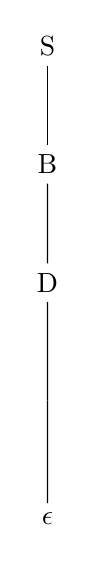
\begin{tikzpicture}
    \node{S}
    child{
        node{B}
        child{
            node{D}
            child{
                child{node{$\eps$}}
            }
        }
    } 
    ;
\end{tikzpicture}\\
\gap
(ii)\\
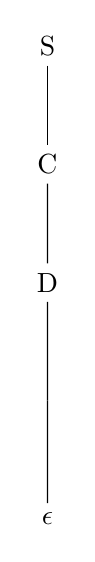
\begin{tikzpicture}
    \node{S}
    child{
        node{C}
        child{
            node{D}
            child{
                child{node{$\eps$}}
            }
        }
    } 
    ;
\end{tikzpicture}\\
\\
$\lightning$ Da die Ableitungsb"aume verschieden sind, ist die Eigenschaft 
    f"ur die Eindeutigkeit von Grammatiken verletzt.\\
\\
Damit ist die Grammatik G mehrdeutig.
\end{document}
